% !TeX root = ../DECO_buku_iot_cerdas.tex
\chapter{ARSITEKTUR SISTEM IOT}

\section{Gambaran Umum Sistem}

Sistem monitoring suhu berbasis IoT cerdas ini terdiri dari empat bagian
utama, yaitu sensor suhu DS18B20, mikrokontroler ESP32-S3, platform
ThingSpeak, dan program AI berbasis Python. Sensor DS18B20 membaca nilai
suhu lingkungan menggunakan komunikasi \textit{1-Wire}
\cite{ds18b20datasheet}. ESP32-S3 kemudian mengambil data suhu tersebut dan
mengirimkannya ke ThingSpeak melalui koneksi Wi-Fi virtual Wokwi. ESP32-S3
mendukung konektivitas Wi-Fi sehingga sesuai digunakan sebagai \textit{node}
IoT pada sistem monitoring berbasis internet \cite{esp32s3espressif}.

ThingSpeak berperan sebagai platform penyimpanan dan visualisasi data. Data
suhu aktual disimpan pada Field~1. Program Python yang berjalan pada Visual
Studio Code membaca data suhu dari ThingSpeak menggunakan \textit{Read API
Key}. Data historis tersebut kemudian diproses menggunakan \textit{Random
Forest Regressor} untuk memprediksi suhu 1 menit ke depan. Hasil prediksi
dikirim kembali ke ThingSpeak pada Field~2, sedangkan status AI dikirim pada
Field~3. Dengan demikian, ThingSpeak berfungsi sebagai penghubung antara
perangkat simulasi IoT dan modul AI di komputer
\cite{thingspeak2024}, \cite{sklearn_rf}.

\section{Komponen Perangkat Keras dan Perangkat Lunak}

Tabel~\ref{tab:komponen} menunjukkan komponen yang digunakan dalam sistem.

\begin{table}[H]
\centering
\caption{Komponen Perangkat Keras dan Perangkat Lunak}
\label{tab:komponen}
\begin{tabularx}{\textwidth}{c L{2.5cm} L{2.8cm} L{6.0cm}}
\toprule
\textbf{No} & \textbf{Komponen} & \textbf{Jenis} & \textbf{Fungsi} \\
\midrule
1  & ESP32       & Mikrokontroler             & Membaca data sensor dan mengirimkan data suhu ke ThingSpeak \\
2  & DS18B20     & Sensor suhu digital        & Mengukur suhu lingkungan berbasis komunikasi \textit{1-Wire} \\
3  & Resistor 4,7\,k$\Omega$ & Komponen pendukung & \textit{Pull-up resistor} antara pin data DS18B20 dan 3,3\,V \\
4  & Wokwi       & Simulator IoT              & Menjalankan simulasi ESP32 dan DS18B20 \\
5  & ThingSpeak  & Platform IoT \textit{cloud} & Menyimpan, menampilkan, dan memvisualisasikan data sensor dan AI \\
6  & VS Code     & IDE                        & Menjalankan program Python AI \\
7  & Python      & Bahasa pemrograman         & Mengolah data historis dan menjalankan model AI \\
8  & scikit-learn & Library \textit{ML}       & Mengimplementasikan \textit{Random Forest Regressor} \\
9  & pandas      & Library Python             & Mengolah data tabular dari ThingSpeak \\
10 & requests    & Library Python             & Melakukan komunikasi HTTP API dengan ThingSpeak \\
\bottomrule
\end{tabularx}
\end{table}

Komponen perangkat keras utama adalah ESP32-S3 dan DS18B20. DS18B20 dipilih
karena mampu menyediakan data suhu digital dan menggunakan antarmuka
\textit{1-Wire} \cite{ds18b20datasheet}. ESP32-S3 dipilih karena mendukung
Wi-Fi 2,4\,GHz sehingga dapat berkomunikasi dengan platform IoT berbasis
internet \cite{esp32s3espressif}. Komponen perangkat lunak utama adalah
ThingSpeak, Wokwi, Python, dan scikit-learn. ThingSpeak digunakan untuk
visualisasi data IoT, Wokwi digunakan sebagai simulator, sedangkan
scikit-learn digunakan untuk membangun model \textit{Random Forest Regressor}
\cite{thingspeak2024}, \cite{wokwi_wifi}, \cite{sklearn_rf},
\cite{pedregosa2011}.

\section{Diagram Blok Sistem}

Sistem memiliki aliran data dari sensor menuju \textit{cloud}, kemudian dari
\textit{cloud} menuju program AI, lalu kembali ke \textit{cloud}. Aliran data
tersebut menunjukkan bahwa sistem berjalan secara \textit{end-to-end}, mulai
dari pembacaan sensor hingga visualisasi hasil prediksi. Diagram blok sistem
terdiri dari lima blok utama, yaitu DS18B20, ESP32-S3, ThingSpeak Field~1,
Python Random Forest, dan ThingSpeak Dashboard (Field~2 dan Field~3).

\begin{figure}[H]
\centering
\begin{tikzpicture}[
    node distance=0.6cm and 1.0cm,
    block/.style={rectangle, draw, rounded corners=3pt, align=center,
                  minimum height=1.2cm, minimum width=2.8cm, font=\small},
    arrow/.style={-Latex, thick}
]
\node[block, fill=blue!15]   (ds18b20)  {DS18B20\\Sensor Suhu};
\node[block, fill=blue!15,   right=of ds18b20] (esp32) {ESP32-S3\\Wokwi};
\node[block, fill=green!15,  right=of esp32]   (ts1)   {ThingSpeak\\Field 1\\Suhu Aktual};
\node[block, fill=orange!15, below=1.6cm of ts1] (ai)  {Python\\Random Forest\\Regressor};
\node[block, fill=green!15,  left=of ai]  (ts23) {ThingSpeak\\Field 2 \& 3\\Prediksi + Status};
\node[block, fill=purple!15, left=of ts23] (dash) {Dashboard\\ThingSpeak\\Visualisasi};

\draw[arrow] (ds18b20) -- node[above,font=\tiny]{1-Wire} (esp32);
\draw[arrow] (esp32)   -- node[above,font=\tiny,align=center]{HTTP POST\\15 det} (ts1);
\draw[arrow] (ts1)     -- node[right,font=\tiny,align=center]{HTTP GET\\10 det} (ai);
\draw[arrow] (ai)      -- node[above,font=\tiny]{HTTP POST} (ts23);
\draw[arrow] (ts23)    -- (dash);
\draw[arrow] (ts1)     -- ++(0,-0.8) -| (dash);
\end{tikzpicture}
\caption{Diagram Blok Sistem Monitoring Suhu Berbasis IoT Cerdas Menggunakan
ESP32-S3, DS18B20, ThingSpeak, dan Random Forest}
\label{fig:diagram-blok}
\end{figure}

\section{Wiring Sistem pada Wokwi}

Sensor DS18B20 dihubungkan ke ESP32-S3 menggunakan protokol \textit{OneWire}.
Pin data sensor dihubungkan ke GPIO4. Pin VCC sensor dihubungkan ke 3V3,
sedangkan GND sensor dihubungkan ke GND ESP32-S3. Resistor 4,7\,k$\Omega$
digunakan sebagai \textit{pull-up resistor} antara pin data dan 3V3.
Penggunaan \textit{pull-up resistor} diperlukan karena komunikasi
\textit{1-Wire} menggunakan jalur data tunggal yang membutuhkan kondisi logika
stabil pada saat tidak ada transmisi data \cite{ds18b20datasheet}.
Konfigurasi pin secara lengkap ditunjukkan pada Tabel~\ref{tab:pin} dan
rangkaian wiring pada simulator Wokwi ditunjukkan pada
Gambar~\ref{fig:wiring-wokwi}.

\begin{table}[H]
\centering
\caption{Konfigurasi Pin ESP32-S3 dan DS18B20}
\label{tab:pin}
\begin{tabularx}{\textwidth}{L{3.5cm} L{3.5cm} L{6.0cm}}
\toprule
\textbf{Pin DS18B20} & \textbf{Pin ESP32} & \textbf{Keterangan} \\
\midrule
VCC              & 3V3                      & Catu daya sensor \\
GND              & GND                      & \textit{Ground} \\
DQ / DATA        & GPIO4                    & Jalur data \textit{1-Wire} \\
DQ / DATA ke 3V3 & Resistor 4,7\,k$\Omega$ & \textit{Pull-up resistor} \\
\bottomrule
\end{tabularx}
\end{table}

\begin{figure}[H]
\centering
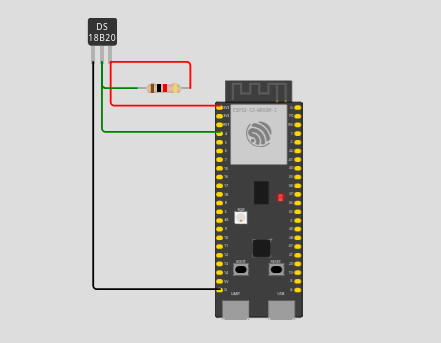
\includegraphics[width=0.55\textwidth]{images/gambar_bab_4/wiringwokwi.png}
\caption{Rangkaian wiring sensor DS18B20 dengan ESP32 pada simulator Wokwi.
Pin data DS18B20 terhubung ke GPIO4 dengan \textit{pull-up} resistor 4,7\,k$\Omega$.}
\label{fig:wiring-wokwi}
\end{figure}

\section{Konfigurasi ThingSpeak}

ThingSpeak digunakan untuk menampilkan data suhu dan hasil AI. Platform ini
mendukung pengumpulan dan visualisasi data IoT dalam bentuk grafik berbasis
\textit{cloud} \cite{thingspeak2024}. Channel ThingSpeak dikonfigurasi dengan
tiga \textit{field} utama, yaitu suhu aktual, prediksi suhu 1 menit ke depan,
dan status AI.

\begin{table}[H]
\centering
\caption{Konfigurasi Field ThingSpeak}
\label{tab:thingspeak}
\begin{tabularx}{\textwidth}{c L{3.5cm} L{2.8cm} L{5.5cm}}
\toprule
\textbf{Field} & \textbf{Nama Field} & \textbf{Sumber Data} & \textbf{Fungsi} \\
\midrule
Field 1 & Temperature                 & ESP32 / Wokwi        & Menampilkan suhu aktual dari DS18B20 \\
Field 2 & Predicted Temperature 1 Min & Python Random Forest & Menampilkan prediksi suhu 1 menit ke depan \\
Field 3 & AI Status Code              & Python Random Forest & Menampilkan status hasil klasifikasi AI \\
\bottomrule
\end{tabularx}
\end{table}

Kode status AI yang digunakan adalah: 0\,=\,Dingin, 1\,=\,Normal, dan
2\,=\,Panas.

\section{Flowchart Sistem}

Alur kerja sistem dimulai dari inisialisasi ESP32-S3, koneksi Wi-Fi,
pembacaan sensor DS18B20, pengiriman data ke ThingSpeak, pembacaan data oleh
Python, pemrosesan Random Forest, pengiriman hasil AI ke ThingSpeak, dan
visualisasi dashboard. Pada Wokwi, koneksi internet ESP32 dilakukan melalui
gateway khusus yang memungkinkan simulasi ESP32 berkomunikasi dengan internet
\cite{wokwi_wifi}.

\begin{figure}[H]
\centering
\begin{tikzpicture}[
    node distance=0.50cm,
    espnode/.style={rectangle, draw, fill=blue!15, minimum width=3.8cm,
                    minimum height=0.65cm, align=center, font=\small},
    ainode/.style={rectangle, draw, fill=orange!15, minimum width=3.8cm,
                   minimum height=0.65cm, align=center, font=\small},
    tsnode/.style={rectangle, draw=green!60!black, fill=green!15,
                   rounded corners=4pt, minimum width=3.8cm,
                   minimum height=0.65cm, align=center, font=\small},
    startstop/.style={ellipse, draw, fill=gray!20, minimum width=3.4cm,
                      minimum height=0.65cm, align=center, font=\small},
    decision/.style={diamond, draw, fill=yellow!20, minimum width=2.8cm,
                     minimum height=0.7cm, align=center, font=\small, aspect=2.2},
    arrow/.style={-Latex, thick}
]

%% ---- Header kolom ----
\node[font=\small\bfseries, color=blue!70!black]   at (-4.3, 1.1) {ALUR ESP32 (Wokwi)};
\node[font=\small\bfseries, color=orange!80!black] at ( 4.3, 1.1) {ALUR PYTHON AI};
\draw[dashed, color=gray!50, thin] (0, 1.3) -- (0, -13.5);

%% ---- KIRI: ESP32 ----
\node[startstop]              (e1) at (-4.3,  0.0)  {Mulai ESP32};
\node[espnode, below=of e1]   (e2)                   {Init ESP32 \& sensor};
\node[espnode, below=of e2]   (e3)                   {Koneksi Wi-Fi\\Wokwi-GUEST};
\node[espnode, below=of e3]   (e4)                   {Baca suhu DS18B20\\(GPIO4, 1-Wire)};
\node[decision, below=of e4]  (e5)                   {Sensor\\valid?};
\node[espnode, below=of e5]   (e6)                   {Kirim suhu ke\\ThingSpeak Field~1};
\node[tsnode,  below=of e6]   (ts1)                  {\textbf{ThingSpeak Field~1}\\HTTP POST / 15 detik};
\node[espnode, below=of ts1]  (e7)                   {Tunggu 15 detik};

\draw[arrow] (e1)--(e2);
\draw[arrow] (e2)--(e3);
\draw[arrow] (e3)--(e4);
\draw[arrow] (e4)--(e5);
\draw[arrow] (e5)--node[right,font=\tiny]{Ya}(e6);
\draw[arrow] (e5.west)--++(-0.9,0)|-node[above,font=\tiny]{Tidak}(e4.west);
\draw[arrow] (e6)--(ts1);
\draw[arrow] (ts1)--(e7);
\draw[arrow] (e7.south)--++(0,-0.4)--++(-1.5,0)|-(e4.west);

%% ---- KANAN: Python AI ----
\node[startstop]              (p1) at ( 4.3,  0.0)  {Mulai Python AI};
\node[tsnode,  below=of p1]   (ts2)                  {\textbf{ThingSpeak Field~1}\\HTTP GET / 10 detik};
\node[ainode,  below=of ts2]  (p2)                   {Ambil 200 data terbaru};
\node[decision, below=of p2]  (p3)                   {Data\\cukup?};
\node[ainode,  below=of p3]   (p4)                   {Buat 7 fitur \textit{time series}};
\node[ainode,  below=of p4]   (p5)                   {Training Random Forest\\(split 80/20)};
\node[ainode,  below=of p5]   (p6)                   {Prediksi suhu\\1 menit ke depan};
\node[ainode,  below=of p6]   (p7)                   {Klasifikasi:\\Dingin / Normal / Panas};
\node[tsnode,  below=of p7]   (ts3)                  {\textbf{ThingSpeak Field~2 \& 3}\\HTTP POST / $\geq$45 detik};
\node[ainode,  below=of ts3]  (p9)                   {Tunggu 10 detik};

\draw[arrow] (p1)--(ts2);
\draw[arrow] (ts2)--(p2);
\draw[arrow] (p2)--(p3);
\draw[arrow] (p3)--node[right,font=\tiny]{Ya}(p4);
\draw[arrow] (p3.east)--++(0.9,0)|-node[above,font=\tiny]{Tidak}(p2.east);
\draw[arrow] (p4)--(p5);
\draw[arrow] (p5)--(p6);
\draw[arrow] (p6)--(p7);
\draw[arrow] (p7)--(ts3);
\draw[arrow] (ts3)--(p9);
\draw[arrow] (p9.east)--++(1.4,0)|-(p2.east);

\end{tikzpicture}
\caption{Flowchart alur kerja sistem monitoring suhu berbasis IoT cerdas. Alur ESP32/Wokwi (kiri, biru) dan alur Python AI (kanan, oranye) berjalan secara paralel dan independen. Kotak hijau menunjukkan interaksi dengan ThingSpeak sebagai platform \textit{cloud} penghubung.}
\label{fig:flowchart}
\end{figure}

\section{Mekanisme Komunikasi Data}

Komunikasi data pada sistem ini dilakukan melalui protokol HTTP API.
ESP32-S3 mengirim data suhu ke ThingSpeak menggunakan \textit{Write API Key}.
Program Python membaca data dari ThingSpeak menggunakan \textit{Read API Key}
dan mengirim hasil prediksi menggunakan \textit{Write API Key}. Dengan
mekanisme ini, ThingSpeak berfungsi sebagai media penyimpanan data sekaligus
perantara komunikasi antara perangkat IoT dan modul AI
\cite{thingspeak2024}.

Pada simulator Wokwi, koneksi Wi-Fi menggunakan SSID virtual
\texttt{Wokwi-GUEST} tanpa \textit{password}. Konfigurasi ini digunakan
karena perangkat ESP32 yang berjalan di \textit{browser} tidak secara
langsung menggunakan jaringan Wi-Fi fisik pengguna, melainkan menggunakan
gateway internet yang disediakan oleh Wokwi \cite{wokwi_wifi}.
